\SubProblem
{بارگذاری فایل فرکانس کلمات و محاسبه هزینه فاصله گذاری}
{
\begin{figure}[H]
    \centering
    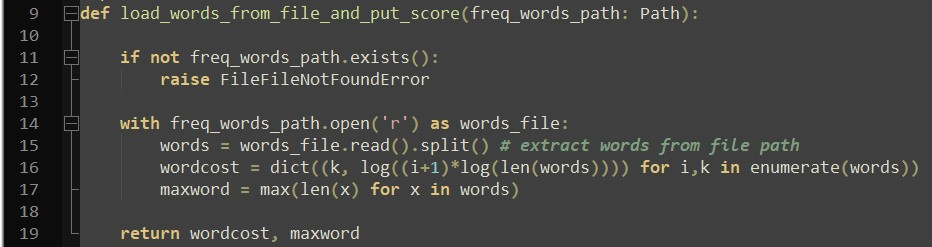
\includegraphics[width=15cm]{Images/F1.jpg}
    \label{fig:label}
    \caption{کد فرکانس کلمات و محاسبه هزینه}
\end{figure}

این تابع فایل تکرار کلمات را بارگذاری می‌کند و بر اساس ترتیب کلمات یک امتیاز یا هزینه نسبت به هر کلمه اختصاص می‌دهد. طبیعتا هر چه تکرار یک کلمه بیشتر باشد برای ما مطلوب‌تر است که آن کلمه را در متن داشته باشیم و اسپیس گذاری را بر مبنای آن انجام می‌دهیم.
}
